\chapter{Lambda Calculus}

\begin{sidenotebox}{Type Systems for Programming Languages}
    The third-year type systems module contains an introduction to lambda calculus that can be found \href{https://oliverkillane.github.io/Imperial-Computing-Notes/60023%20-%20Type%20Systems%20for%20Programming%20Languages/}{here}. 
\end{sidenotebox}

\section{Lambda Calculus}
\begin{center}
    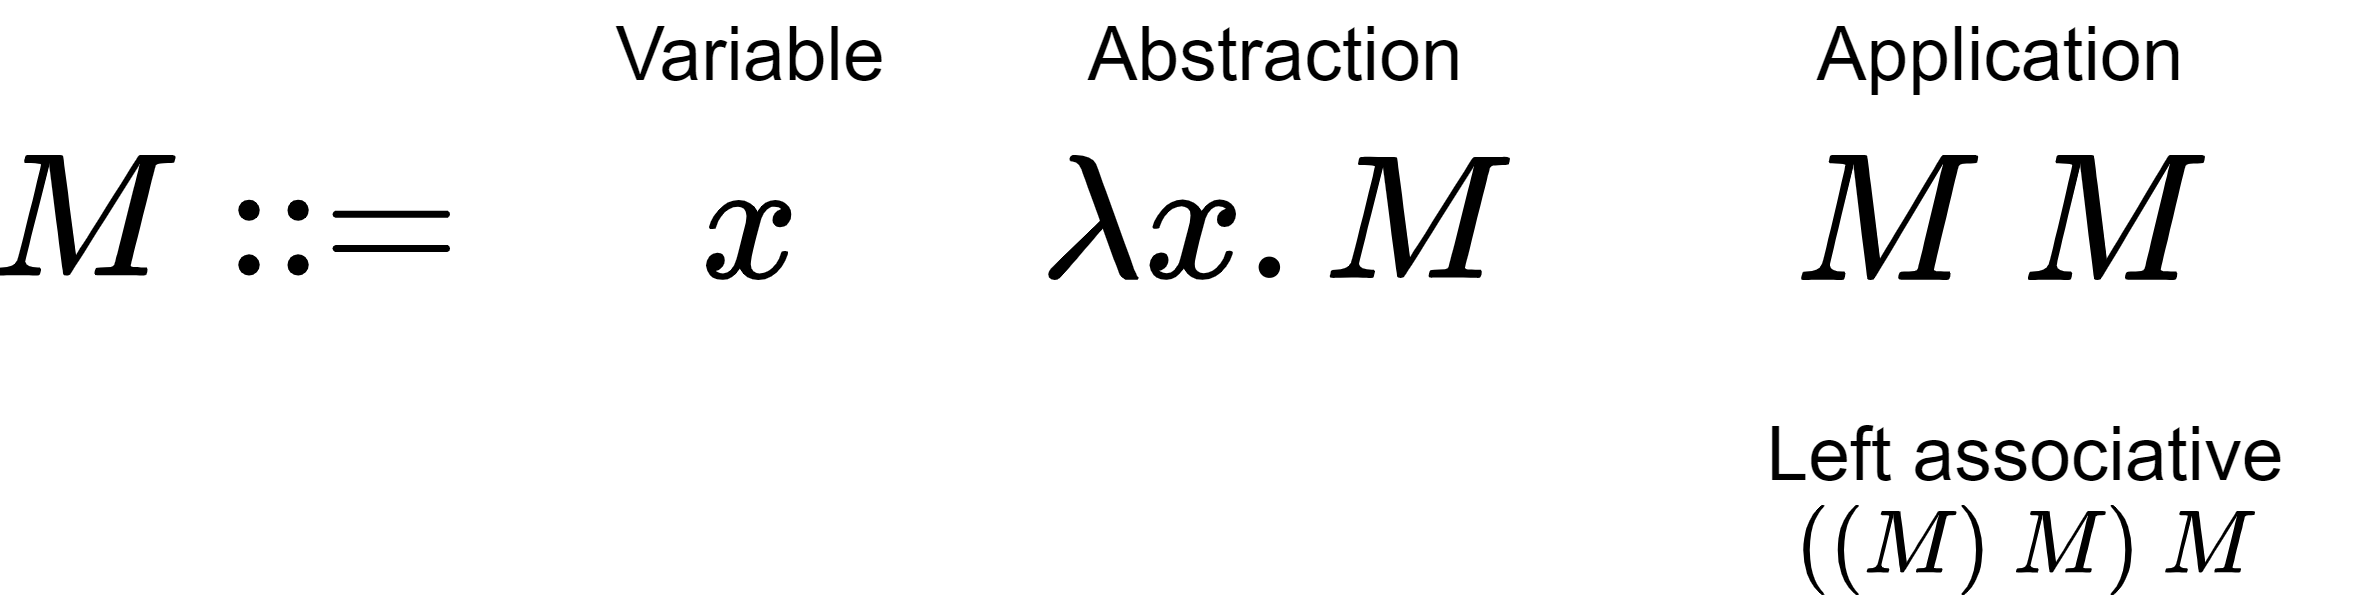
\includegraphics[width=0.7\textwidth]{lambda_calculus/images/lambda_form.drawio.png}
\end{center}

\section{Syntax}
\begin{center}
    \begin{tabular}{l p{.8\textwidth}}
        \textbf{Bound Variables} & $x$ is bound inside $\lambfun{x}{M}$ (it is bound within the scope of $M$) \\
        \textbf{Free Variables} & $y$ is free inside $\lambfun{x}{M}$ (it is not bound) \\
        \textbf{Closed Term} & A $\lambda$-term with no free variables, e.g $\lambfun{\lambarg{x}{y}{z}}{x \ y}$ \\
        \textbf{Binding Occurences} & The $\lambda$-term's parameters $\lambfun{\lambarg{x}{y}{z}}{(\dots)}$, here the $x$, $y$ and $z$ before the dot. \\
        \textbf{Left Associativity} & Lambda Terms are left associative, hence $\lambapp{\lambapp{\lambapp{A}{B}}{C}}{D} \equiv \lambappb{\lambappb{\lambappb{A}{B}}{C}}{D}$ \\
    \end{tabular}
\end{center}

\subsection{Bound and Free Formally}
\[\begin{matrix*}[l]
		FreeVariables & (x) &=  \{x\} \\
		FreeVariables & (\lambfun{x}{M}) &= FreeVariables(M) \setminus \{x\} \\
		FreeVariables & (M \ N) &= FreeVariables(M) \cup FreeVariables(N) \\
	\end{matrix*}\]

\begin{definitionbox}{$\alpha$-equivalence}
	\[M =_\alpha N \ \text{ if and only if $N$ can be obtained from $M$ by renaming bound variables (or vice-versa)}\]
	Hence the free variable set must be the same (not renamed).
\end{definitionbox}

\subsection{Substitution}
\[M [new / old] \text{ means replace free variable $old$ with $new$ in $M$}\]
Only free variables can be substituted.
Formally we can describe this as:
\[\begin{split}
		x[M/y] &= \begin{cases}
			M & x = y    \\
			x & x \neq y \\
		\end{cases} \\
		(\lambfun{x}{N})[M/y] &= \begin{cases}
			\lambfun{x}{N}           & x = y \ \text{($x$ will be bound inside, so cannot go further)}                                                   \\
			\lambfun{z}{N[z/x][M/y]} & x \neq y \ \text{(To avoid name conflicts with $M$, $z \not\in ((FV(N) \setminus \{x\}) \cup FV(M) \cup \{y\})$)}
		\end{cases} \\
		(\lambapp{A}{B})[M/y] &= \lambappb{A[M/y]}{B[M/y]} \\
	\end{split}\]
\begin{itemize}
	\item For variables, simply check if equal.
	\item For lambda abstractions, if the old term is bound, cannot go further, else, switch the bound term for some term not free inside, in the substitution, and not the new value replacing.
	\item For applications, simply substitute into both $\lambda$-terms.
\end{itemize}

\begin{examplebox}{Basic Substitution}
	\[\begin{split}
			x[y/x] &= y \\
			y[y/x] &= y \\
			(\lambapp{x}{y})[y/x] &= \lambapp{y}{y} \\
			\lambfun{x}{\lambapp{x}{y}}[y/x] &= \lambfun{x}{\lambapp{x}{y}} \\
		\end{split}\]
\end{examplebox}

\section{Semantics}
\[\begin{matrix}
		\cfrac{}{\lambapp{(\lambfun{x}{M})}{N} \to_\beta M[N/x]}         &
		\cfrac{M \to_\beta M'}{\lambfun{x}{M} \to_\beta \lambfun{x}{M'}} &
		\cfrac{M \to_\beta M'}{\lambapp{M}{N} \to_\beta \lambapp{M'}{N}} &
		\cfrac{N \to_\beta N'}{\lambapp{M}{N} \to_\beta \lambapp{M}{N'}}   \\
	\end{matrix}
\]
\[\cfrac{M =_\alpha M' \ M' \to_\beta N' \ N' =_\alpha N }{M \to_\beta N}\]

\begin{itemize}
	\item A term of the form $\lambapp{(\lambfun{x}{N}) \ M}$ is called a \textit{redex}.
	\item A $\lambda$-term may have several different reductions. These different reductions for a \textit{derivation tree}.
\end{itemize}

\subsection{Multi-Step Reductions}
Steps can be combined using the transitive closure of $\to_\beta$ under $\alpha$-conversion.
\[\begin{matrix}
		\cfrac{M =_\alpha M'}{M \to^*_\beta M'}                        & \text{  (Reflexivity of $\alpha$-conversion)} \\
		\\
		\cfrac{M \to_\beta M' \ M' \to^*_\beta M''}{M \to^*_\beta M''} & \text{  (Transitivity)}                       \\
	\end{matrix}\]

\begin{definitionbox}{Confluence}
All derivation paths in the derivation tree that reach some normal form, reach the same normal form.
\[\forall M, M_1, M_2. \ [M \to^*_\beta M_1 \land M \to^*_\beta M_2 \Rightarrow \exists M'. [M_1 \to^*_\beta M' \land M_2 \to^*_\beta M']]\]
    \begin{center}
        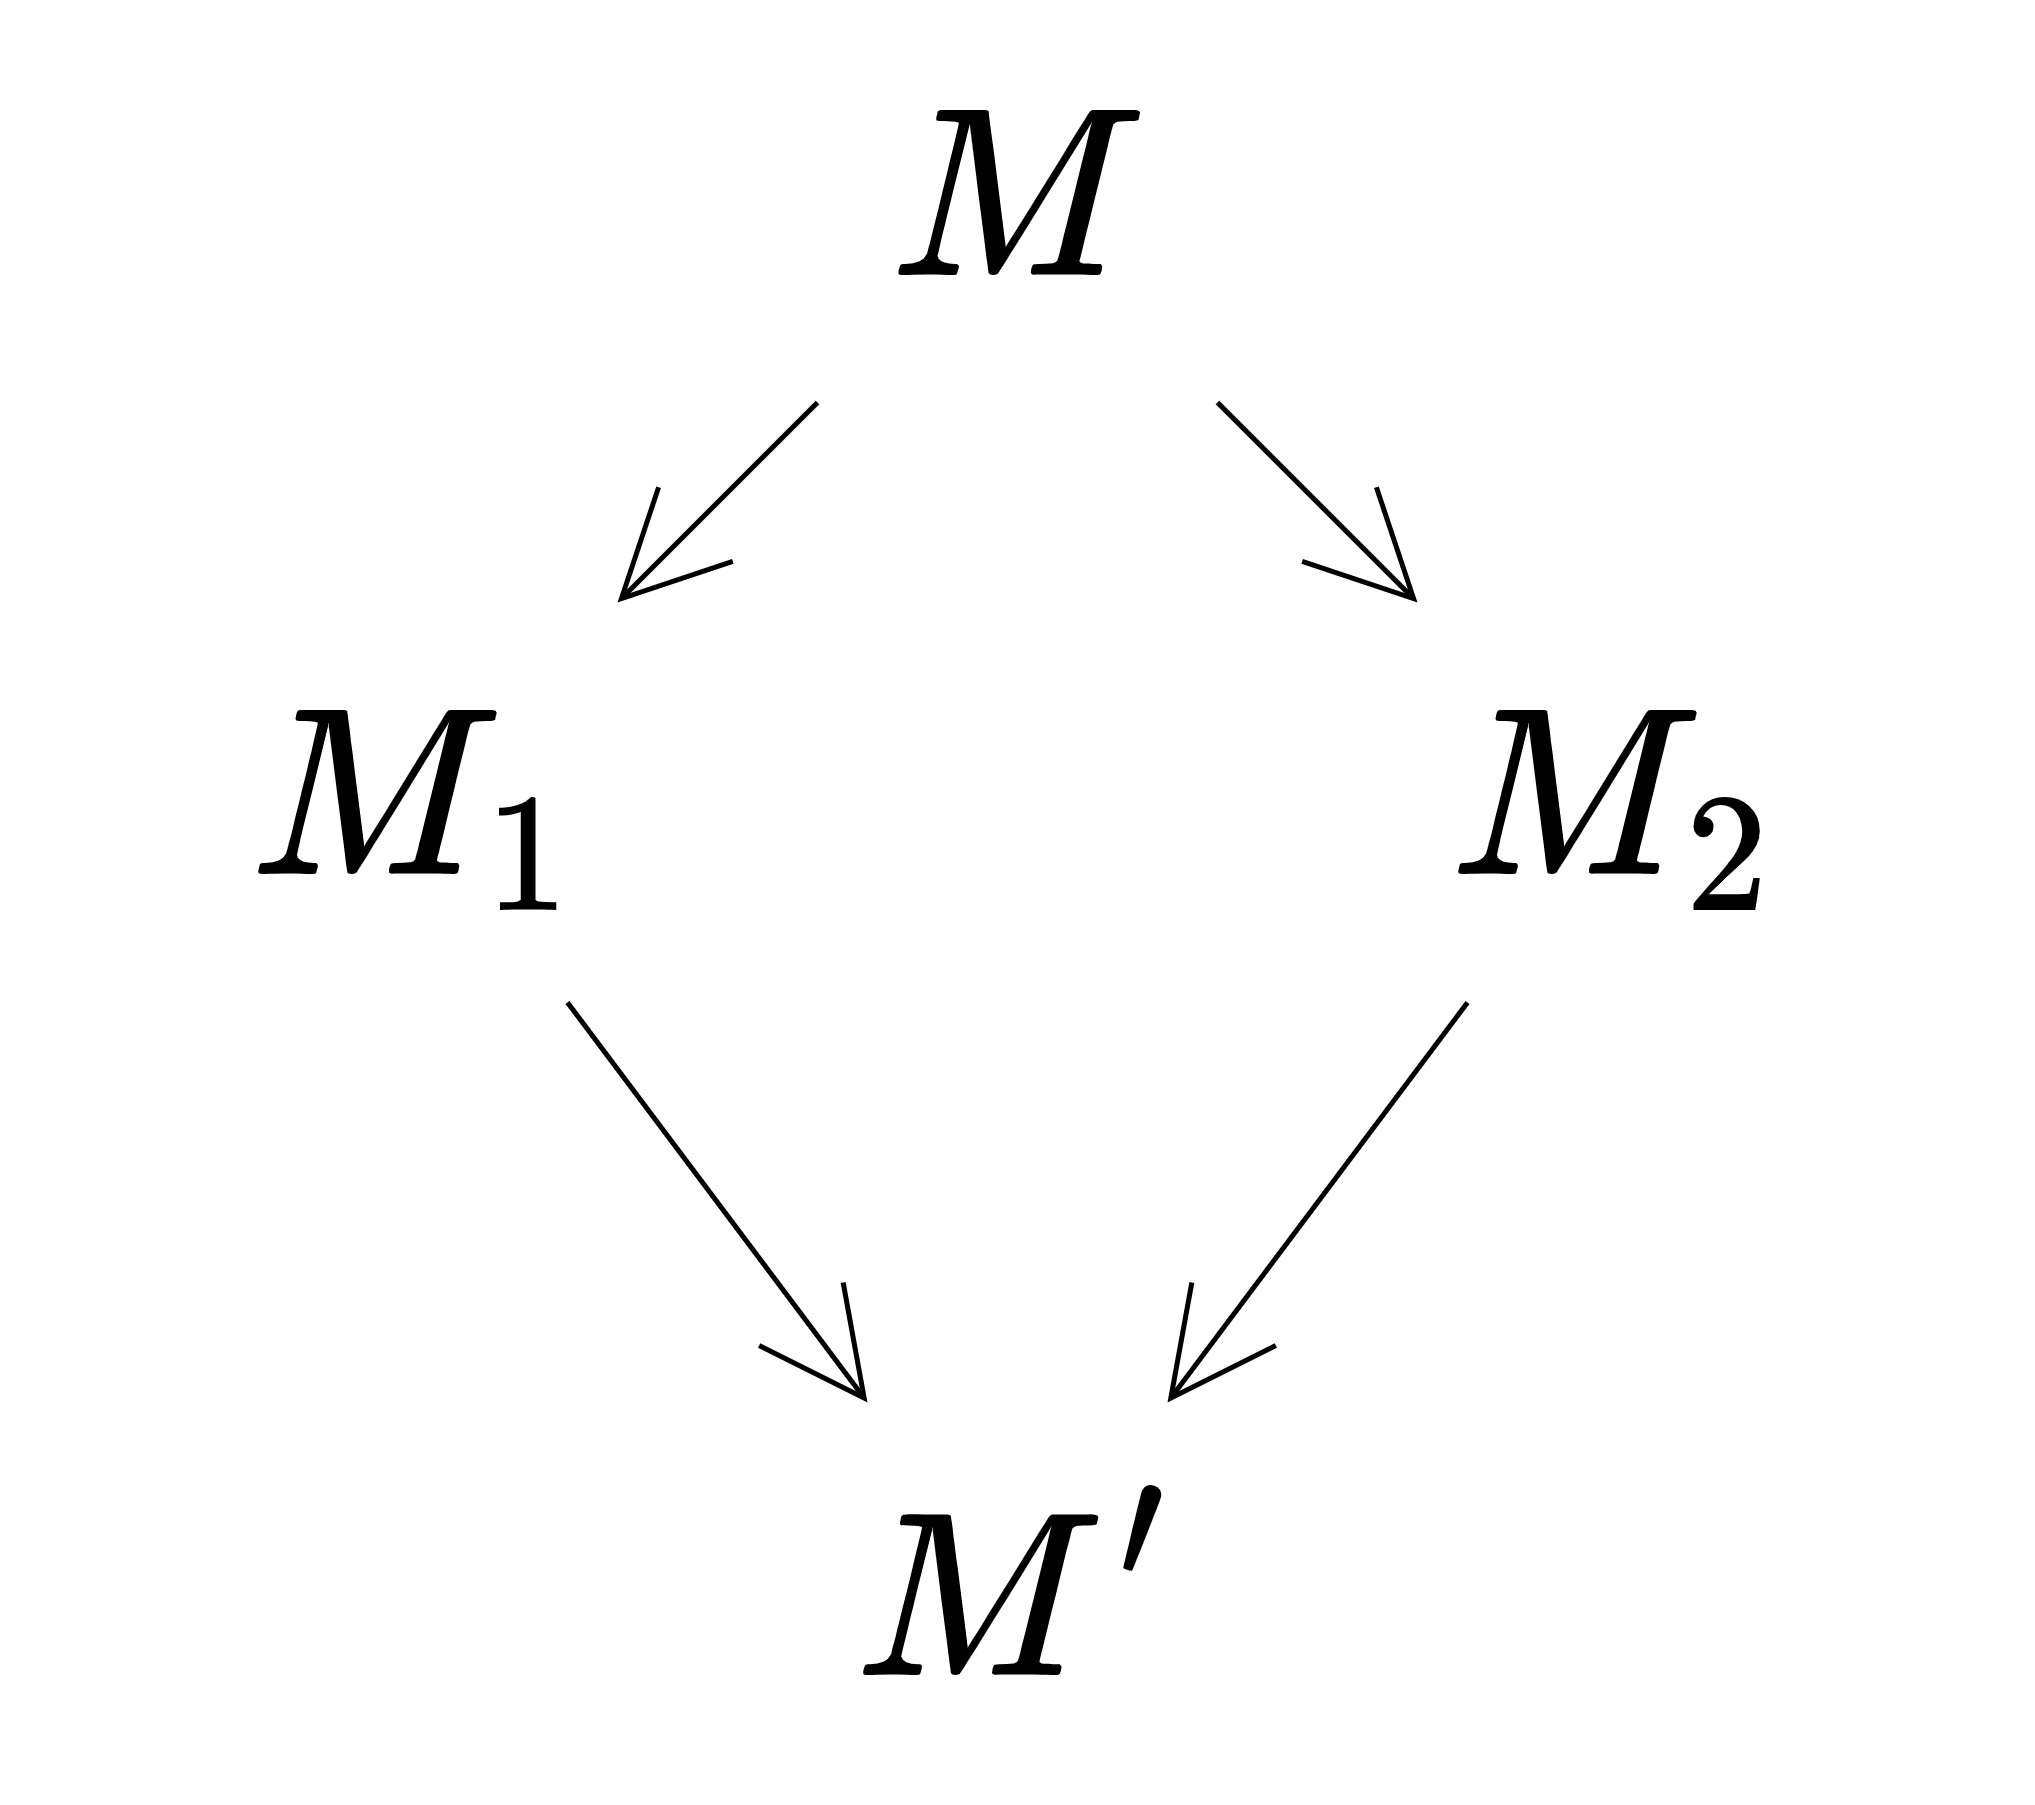
\includegraphics[width=0.3\textwidth]{lambda_calculus/images/confluence.drawio.png}
    \end{center}
\end{definitionbox}

\begin{definitionbox}{$\beta$ Normal Forms}
A $\lambda$-term is in $\beta$-normal form if it contains no \textit{redexes}, and hence cannot be further reduced.
\[\begin{split}
		\text{is in normal form}(M) &\triangleq \forall N. \ M \not\to_\beta N \\
		\text{has a normal form}(M) &\triangleq \exists M'. \ M \to^*_\beta M' \land \text{is in normal form}(M) \\
	\end{split}\]
If a normal form exists, it is unique.
\[\forall M, N_1, N_2, . \ [M \to^*_\beta N_1 \land M \to^*_\beta N_2 \land \text{is-norm-form}(N_1) \land \text{is-norm-form}(N_2) \Rightarrow N_1 =_\alpha N_2]\]
\end{definitionbox}
\begin{definitionbox}{$\beta$-equivalence}
An equivalence relation for $\to_\beta$.
\[M =_\beta N \Leftrightarrow \exists T. \ [M \to^*_\beta T \land N \to^*_\beta T]\]
\end{definitionbox}

\subsection{Reduction Order}

For a \textit{redex} $E = \lambapp{(\lambfun{x}{M})}{N}$:
\begin{itemize}
	\item Any \textit{redex} in $M$ or $N$ is inside of $E$
	\item $E$ is outside of any \textit{redex} in $M$ or $N$
\end{itemize}
\begin{tcbraster}[raster columns=2,raster equal height]
\begin{definitionbox}{Innermost Redex}
	A \textit{Redex} with no \textit{redexes} inside of it.
\end{definitionbox}
\begin{definitionbox}{Outermost Redex}
	A \textit{Redex} with no \textit{redexes} outside of it.
\end{definitionbox}
\end{tcbraster}
We can choose several different orders by which to reduce.
\begin{definitionbox}{Normal Order}
    \begin{itemize}
        \item Reduce the \textit{leftmost outermost} \textit{redex} first.
        \item This always reduces a $\lambda$-term to its normal form if one exists.
        \item Can perform computations on unevaluated function bodies.
        \item Not used in any programming languages.
    \end{itemize}
\end{definitionbox}
\begin{definitionbox}{Call By Name}
    \begin{itemize}
        \item Reduce the \textit{leftmost outermost} first.
        \item Does not reduce the inside of $\lambda$-abstractions.
        \item Does not always reduce a $\lambda$-term to its normal form.
        \item Passes unevaluated function parameters into function body. Only evaluating a parameter when it is used.
        \item Used with some variation by haskell, R, and \LaTeX.
    \end{itemize}
\end{definitionbox}
\begin{definitionbox}{Call By Values}
    \begin{itemize}
        \item Reduce the \textit{leftmost innermost} \textit{redex} first.
        \item Does not reduce the inside of $\lambda$-abstractions.
        \item Does not always reduce a $\lambda$-term to its normal form.
        \item Evaluate parameters before passing them to function body.
        \item Terminates less often than \textit{call by name} (e.g if a parameter cannot be normalised, but is never used), but evaluated the parameters only once.
        \item Used by C, Rust, Java, etc.
    \end{itemize}
\end{definitionbox}

\begin{definitionbox}{$\eta$-equivalence}
Captures equality better than $=_\beta$.
\[\begin{matrix}
        \cfrac{x \not\in FV(M)}{\lambfun{x}{\lambapp{M}{x}} =_\eta M} & \cfrac{\forall N. \ \lambapp{M}{N} =_{\eta^+} \lambapp{M'}{N}}{M =_{\eta^+} M'}
    \end{matrix}\]
Namely if the application of $M$ to another $\lambda$-term is equivalent to $M'$ applied to the same $\lambda$-terms then $M$ and $M'$ are equivalent.
\\
\\ For example with the basic application of $f$:
\[\begin{matrix}
        \lambfun{x}{\lambapp{f}{x}} \neq_\beta f & \text{  however  } & \lambapp{(\lambfun{x}{\lambapp{f}{x}})}{M} =_\beta \lambapp{f}{M} & \text{  and  } & \lambfun{x}{\lambapp{f}{x}} \neq_\eta f \\
    \end{matrix}\]
\end{definitionbox}

\subsection{Definability}
\begin{definitionbox}{$\lambda$-definable}
	Partial function $f: \mathbb{N}^n \rightharpoonup \mathbb{N}$ is \textit{$\lambda$-definable} if and only if there is a \textit{closed} $\lambda$-term $M$ where:
	\[f(x_1, \dots, x_n) = y \Leftrightarrow \lambapp{\lambapp{\lambapp{M}{\underline{x_1}}}{\dots}}{\underline{x_n}} =_\beta y\]
	And
	\[f(x_1, \dots, x_n)\uparrow \Leftrightarrow \lambapp{\lambapp{\lambapp{M}{\underline{x_1}}}{\dots}}{\underline{x_n}} \text{  has no \textit{normal form}}\]
\end{definitionbox}

\textit{$\lambda$-definable} specifies what can be computed by the lambda calculus, and is equivalent to \textit{Register Machine Computable} or \textit{Turing Machine Computable}.

\section{Encoding Mathematics}
\subsection{Encoding Numbers}
We represent natural numbers as \textit{Church Numerals}. These are $n$ repeated applications of some function $f$.
\[\underline{n} \triangleq \lambfun{f}{\lambfun{x}{\underbrace{f(\dots (\lambapp{f}{x})}_\text{$n$ times} \dots )}} \text{  with $n$ applications of $f$}\]
\[\begin{split}
    \chnum{0} &\triangleq \lambfun{f}{\lambfun{x}{x}} \\
    \chnum{1} &\triangleq \lambfun{f}{\lambfun{x}{\lambapp{f}{x}}} \\
    \chnum{2} &\triangleq \lambfun{f}{\lambfun{x}{\lambapp{f}{\lambapp{f}{x}}}} \\
    \chnum{3} &\triangleq \lambfun{f}{\lambfun{x}{\lambapp{f}{\lambapp{f}{\lambapp{f}{x}}}}} \\
    \chnum{4} &\triangleq \lambfun{f}{\lambfun{x}{\lambapp{f}{\lambapp{f}{\lambapp{f}{\lambapp{f}{x}}}}}} \\
    \chnum{5} &\triangleq \lambfun{f}{\lambfun{x}{\lambapp{f}{\lambapp{f}{\lambapp{f}{\lambapp{f}{\lambapp{f}{x}}}}}}} \\
    \vdots \\
\end{split}\]

\subsection{Encoding Addition}
Addition is represented as a function application:
\[\begin{matrix}
		\underline{m} =  \lambfun{f}{\lambfun{x}{\underbrace{f(\dots (\lambapp{f}{x})}_\text{$m$ times} \dots )}} & \underline{n} =  \lambfun{f}{\lambfun{x}{\underbrace{f(\dots (\lambapp{f}{x})}_\text{$n$ times} \dots )}} \\
	\end{matrix}\]
\[\underline{m + n} \triangleq \lambapp{\lambapp{\underbrace{(\lambfun{m}{\lambfun{n}{\lambfun{f}{\lambfun{x}{\lambapp{\lambapp{m}{f}}{(\lambapp{\lambapp{n}{f}}{x})}}}}})}_+}{\underline{m}}}{\underline{n}}\]
By applying the functions, we have $f$ applied $m + n$ times, representing the \textit{Church Numeral} $\underline{m+n}$.

\subsection{Encoding Multiplication}
\[\begin{matrix}
		\underline{m} =  \lambfun{f}{\lambfun{x}{\underbrace{f(\dots (\lambapp{f}{x})}_\text{$m$ times} \dots )}} & \underline{n} =  \lambfun{f}{\lambfun{x}{\underbrace{f(\dots (\lambapp{f}{x})}_\text{$n$ times} \dots )}} \\
	\end{matrix}\]
\[\underline{m \times n} \triangleq \lambapp{\lambapp{\underbrace{(\lambfun{m}{\lambfun{n}{\lambfun{f}{\lambapp{m}{(\lambapp{n}{f})}}}})}_\times}{\underline{m}}}{\underline{n}}\]
Each application of the $f$ inside $m$ is substituted for $n$ applications of $f$, using the above $\lambda$-abstraction we get $m \times n$ applications of $f$.
\subsection{Exponentiation}
\[\begin{matrix}
		\underline{m} =  \lambfun{f}{\lambfun{x}{\underbrace{f(\dots (\lambapp{f}{x})}_\text{$m$ times} \dots )}} & \underline{n} =  \lambfun{f}{\lambfun{x}{\underbrace{f(\dots (\lambapp{f}{x})}_\text{$n$ times} \dots )}} \\
	\end{matrix}\]
\[\underline{m^n} \triangleq \lambapp{\lambapp{\underbrace{(\lambfun{m}{\lambfun{n}{\lambapp{n}{m}}})}_\text{exponential}}{\underline{m}}}{\underline{n}}\]
\subsection{Conditional}
\[\underline{m} =  \lambfun{f}{\lambfun{x}{\underbrace{f(\dots (\lambapp{f}{x})}_\text{$m$ times} \dots )}}\]
\[\text{if $m = 0$ then $x_1$ else $x_2$} \triangleq \lambapp{\underbrace{(\lambfun{m}{\lambfun{x_1}{\lambfun{x_2}{\lambapp{\lambapp{m}{(\lambfun{z}{x_2})}}{x_1}}}})}_\text{if zero}}{\underline{m}}\]
If $\underline{m} = \chnum{0} = \lambfun{f}{\lambfun{x}{x}}$ then $x$ is returned, which will be $x_1$.
\\
\\ If not zero, then the $f$ applied returns $x_2$, so any number of applications of $f$, results in $x_2$.
\subsection{Successor}
\[\underline{m} =  \lambfun{f}{\lambfun{x}{\underbrace{f(\dots (\lambapp{f}{x})}_\text{$m$ times} \dots )}}\]
We simply take $\underline{m}$ and apply $f$ one more time
\[\underline{m + 1} \triangleq \lambapp{\underbrace{(\lambfun{m}{\lambfun{f}{\lambfun{x}{\lambapp{f}{(\lambapp{\lambapp{m}{f}}{x})}}}})}_\text{succ}}{\underline{m}}\]

\subsection{Pairs}
We can encode pairs as a function, with a selector $s$ function. Hence by supplying $first$ or $second$ as the selector, we can use the pair.
\[\begin{split}
		newpair(a,b) &\triangleq \lambapp{\lambapp{\underbrace{(\lambfun{a}{\lambfun{b}{\lambfun{s}{\lambapp{\lambapp{s}{a}}{b}}}})}_\text{newpair}}{a}}{b} \equiv \lambapp{\lambapp{\underbrace{(\lambfun{\lambarg{a}{b}{s}}{\lambapp{\lambapp{s}{a}}{b}})}_\text{newpair}}{a}}{b}\\
		first(p) &\triangleq \lambapp{p}{\underbrace{(\lambfun{x}{\lambfun{y}{x}})}_\text{first}} \equiv \lambapp{p}{\underbrace{(\lambfun{\lambarg{x}{y}}{x})}_\text{first}} \\
		second(p) &\triangleq \lambapp{p}{\underbrace{(\lambfun{x}{\lambfun{y}{y}})}_\text{second}} \equiv \lambapp{p}{\underbrace{(\lambfun{\lambarg{x}{y}}{y})}_\text{second}}\\
	\end{split}\]

\begin{exambox}{2bv}{2020/21}
	\textit{\dots continued from 2bvi - 2020/21}
	\\
	\\ Using Church numerals, give an equivalent $\lambda$-term (program) C, i.e. for all $n > 0$ we have $C \ \underline{n} \to_\beta^* \underline{m} $ if and only if the execution of register machine $K$ also halts with $R_0 = m$ when started with $R_0 = n$.
	\\
	\\ You can use the pre-defined operations from the lecture ($plus$, $mult$, $succ$,
	$pred$, $ifz$, etc.) and also integer division ($div$) and reminder ($rem$). It helps to
	use various subroutines.
\end{exambox}

\begin{exambox}{2d}{2021/22}
	Consider the following recursively defined sequence of integers $x_i$:
	\[\begin{split}
		x_0 & = x _ 1 = 1 \\
		x_i & = x_{i-2}^2 + 2 x_{i-1} \\
	\end{split}\]
	Implement this in the $\lambda$-calculus using Church numerals, i.e. write a lambda term $f$ such that $f \ \underline{n}$ reduces to $\underline{x_n}$.
	\\
	\\ You can use functions defined in the lecture, e.g $plus$, $mult$, $ifz$ etc. It might help to define subroutines.
	\\
	\\ Sketch the execution of $f \ \underline{2}$ (you can use $\to_\beta^*$ rather than $\to_\beta$).
\end{exambox}

\subsection{Predecessor}
\[\underline{m} =  \lambfun{f}{\lambfun{x}{\underbrace{f(\dots (\lambapp{f}{x})}_\text{$m$ times} \dots )}}\]
We cannot remove applications of $f$, however we can use a pair to count up until the successor is $\underline{m}$.
\\
\\ Hence we first need a function to get the next pair from the current:
\[\lambapp{transition}{p} \triangleq \lambapp{\underbrace{(\lambfun{n}{\lambapp{\lambapp{newpair}{(\lambapp{second}{n})}}{((\lambapp{second}{n}) + 1)}})}_\text{transition function}}{p}\]
We can then simply run the transition $n$ times on a pair starting by using $f = transition$ and $x = \lambapp{\lambapp{newpair}{\chnum{0}}}{\chnum{0}}$.
\[pred(n) \triangleq \begin{cases}
		0     & n = 0     \\
		n - 1 & otherwise \\
	\end{cases}\]
\[pred(n) \triangleq \lambapp{\underbrace{(\lambfun{n}{\lambapp{\lambapp{\lambapp{n}{transition}}{(\lambapp{\lambapp{newpair}{\chnum{0}}}{\chnum{0}})}}{first}})}_\text{predecessor}}{\underline{n}}\]
A simpler definition of predecessor is:
\[pred(n) \triangleq \lambapp{\underbrace{(\lambfun{n}{\lambfun{f}{\lambfun{x}{\lambapp{\lambapp{\lambapp{n}{(\lambfun{g}{\lambfun{h}{\lambapp{h}{(\lambapp{g}{f})}}})}}{(\lambfun{u}{x})}}{(\lambfun{u}{u})}}}})}_\text{predecessor}}{\chnum{n}}\]

\subsection{Subtraction}
We can use the predecessor function for subtraction. By applying the predecessor function $\chnum{n}$ times on some number $\chnum{m}$ we get $\chnum{m - n}$.
\[\chnum{m - n} \triangleq \lambapp{\lambapp{\underbrace{(\lambfun{m}{\lambfun{n}{\lambapp{\lambapp{m}{pred}}{n}}})}_\text{subtract}}{\chnum{m}}}{\chnum{n}}\]

\section{Combinators}
\begin{definitionbox}{Combinator}
	A \textit{closed} $\lambda$-term (no free variables), usually denoted by capital letters that describe
\end{definitionbox}
\begin{center}
	\begin{tabular}{r c l r c l }
		$I $  & $\triangleq $ & $\lambfun{x}{x}$                                                                                                    & $I(x) $      & $\triangleq$ & $ x$                                              \\
		$K $  & $\triangleq $ & $\lambfun{\lambarg{x}{y}}{x}$                                                                                       & $K(x,y) $    & $\triangleq$ & $ x$                                              \\
		$S $  & $\triangleq $ & $\lambfun{\lambarg{x}{y}{z}}{\lambapp{\lambapp{x}{z}}{(\lambapp{y}{z})}}$                                           & $S(x,y,z) $  & $\triangleq$ & $ x(z)(y(z))$                                     \\
		$T $  & $\triangleq $ & $\lambfun{\lambarg{x}{y}}{\lambapp{y}{x}}$                                                                          & $T(x,y) $    & $\triangleq$ & $ y(x)$                                           \\
		$C $  & $\triangleq $ & $\lambfun{\lambarg{x}{y}{z}}{\lambapp{\lambapp{x}{z}}{y}}$                                                          & $C(x,y,z) $  & $\triangleq$ & $ x(z)(y)$                                        \\
		$V $  & $\triangleq $ & $\lambfun{\lambarg{x}{y}{z}}{\lambapp{\lambapp{z}{x}}{y}}$                                                          & $V(x,y,z) $  & $\triangleq$ & $ z(x)(y)$                                        \\
		$B $  & $\triangleq $ & $\lambfun{\lambarg{x}{y}{z}}{\lambapp{x}{(\lambapp{y}{z})}}$                                                        & $B(x,y,z) $  & $\triangleq$ & $ x(y(z))$                                        \\
		$B' $ & $\triangleq $ & $\lambfun{\lambarg{x}{y}{z}}{\lambapp{y}{(\lambapp{x}{z})}}$                                                        & $B'(x,y,z) $ & $\triangleq$ & $ y(x(z))$                                        \\
		$W $  & $\triangleq $ & $ \lambfun{\lambarg{x}{y}}{\lambapp{\lambapp{x}{y}}{y}}$                                                            & $W(x,y)$     & $\triangleq$ & $x(y)(y)$                                         \\
		$Y$   & $\triangleq$  & $\lambfun{g}{\lambapp{(\lambfun{x}{\lambapp{g}{(\lambapp{x}{x})}})}{(\lambfun{x}{\lambapp{g}{(\lambapp{x}{x})}})}}$ & $Y(f) $      & $\triangleq$ & $ (\lambda x \to f(x(x)))(\lambda x \to f(x(x)))$
	\end{tabular}
\end{center}
Only $SKI$ are required to define any \textit{computable function} (can remove even $\lambda$-abstraction, this is called \textit{$SKI$-Combinator Calculus}).
\\
\\ The $Y$-Combinator is used for recursion. In one step of $\beta$-reduction:
\[\lambapp{Y}{f} \to_\beta \lambapp{f}{(\lambapp{Y}{f})}\]
We cannot define $\lambda$-terms in terms of themselves, as the $\lambda$-term is not yet defined, and infinitely large $\lambda$-terms are not allowed.
\\
\\ We can use the $Y-Combinator$ to create recursion in the absence of recursive $\lambda$-term definitions.
\begin{definitionbox}{Fixed-Point Combinator}
	A higher order function (e.g $fix$) that returns some function of itself:
	\[\begin{split}
			fix \ f &= f(fix \ f) \\
			fix \ f &= f(f(\dots f(fix \ f) \dots)) \text{  (after repeated application)}\\
		\end{split}\]
\end{definitionbox}
\begin{examplebox}{Factorial}
	\[fact(n) = \begin{cases}
			1                  & n = 0     \\
			n \times fact(n-1) & otherwise \\
		\end{cases}\]
	If recursive definitions for $\lambda$-terms were allows, we could express this as:
	\[\begin{split}
			fact &\triangleq \lambfun{n}{\lambapp{\lambapp{\lambapp{\text{if zero}}{n}}{\chnum{1}}}{(\lambapp{\lambapp{multiply}{n}}{(\lambapp{fact}{(\lambapp{pred}{n})})})}} \\
			&\triangleq \lambapp{(\lambfun{f}{\lambfun{n}{\lambapp{\lambapp{\lambapp{\text{if zero}}{n}}{\chnum{1}}}{(\lambapp{\lambapp{multiply}{n}}{(\lambapp{f}{(\lambapp{pred}{n})})})}}})}{fact} \\
		\end{split}\]
	Since we can use the above form (higher order function applied to itself) with the $Y$ combinator.
	\[fact \triangleq Y(\lambfun{f}{\lambfun{n}{\lambapp{\lambapp{\lambapp{\text{if zero}}{n}}{\chnum{1}}}{(\lambapp{\lambapp{multiply}{n}}{(\lambapp{f}{(\lambapp{pred}{n})})})}}}) \]
\end{examplebox}

\begin{exambox}{2c}{2020/21}
	Consider the term $\mathbf{Y}' = \mathbf{UU}$ with $\mathbf{U} = \lambfun{\lambarg{u}{x}}{\lambapp{x}{uux}}$.
	\\
	\\ Why is $\mathbf{Y}$ (and $\mathbf{U}$) a combinator? Show that it is an alternative implementation of the \textit{fixed-point combinator}.
\end{exambox}
